\documentclass[a4paper,12pt]{article}
\usepackage{standalone}
\usepackage[a4paper, top=0.8in, bottom=0.7in, left=0.8in, right=0.8in]{geometry}
\usepackage{amsmath, amsfonts, latexsym, graphicx, fancyhdr, enumitem, setspace, tcolorbox, tikz, multicol, hyperref, xcolor}
\usepackage[defaultfam,tabular,lining]{montserrat}


\hypersetup{
    colorlinks=true,
    linkcolor=blue,
    urlcolor=blue,
    filecolor=blue,
    menucolor=blue,
}


\sloppy

\title{}
\date{}
\hyphenpenalty=10000
\exhyphenpenalty=10000

\setlength{\parindent}{0pt}
\pagestyle{fancy}

\setlength{\headheight}{27.11148pt}
\addtolength{\topmargin}{-15.11148pt}

% Change these commands to update throughout the document
\newcommand{\standards}{CCSS}    % Standard Set (e.g., CCSS, Georgia)
\newcommand{\subject}{Math}      % Subject Name
\newcommand{\levelLetter}{I}     % Curriculum Level (Grade 7)
\newcommand{\doctype}{SWB}       % Document Type (SWB, TWB, etc.)

% Document Title Command
\newcommand{\doctitle}{\standards\ \subject\ Curriculum \levelLetter\ \doctype}

\fancyhf{}
\fancyhead[L]{\textbf{\doctitle}}
\fancyhead[R]{
\includegraphics[width=0.8cm]{Round Logo.png}} % Placeholder for logo
\fancyfoot[C]{\footnotesize \textcopyright{} Study Smart Tutors}
\fancyfoot[R]{\thepage}  % Page number in bottom right corner
\fancyfoot[L]{\hyperlink{toc}{Back to Contents}} % Clickable link in bottom left to TOC

% Reset page numbers after TOC
\newcommand{\startPageNumbers}{\setcounter{page}{1}}

\sloppy



\begin{document}

% Title Page
\pagenumbering{gobble}
\documentclass[12pt]{article}
\usepackage[a4paper, top=0.8in, bottom=0.7in, left=0.8in, right=0.8in]{geometry}
\usepackage{amsmath}
\usepackage{amsfonts}
\usepackage{latexsym}
\usepackage{graphicx}
\usepackage{tikz}
\usepackage{fancyhdr}
\usepackage{tcolorbox}
\usepackage{multicol}
\usepackage{tgadventor}
\renewcommand{\familydefault}{\sfdefault}
\usepackage{enumitem}
\usepackage{setspace}
\setlength{\parindent}{0pt}
\pagestyle{fancy}
\usepackage{needspace}


% Define a new command for the level letter
\newcommand{\levelLetter}{I}  % Change this letter to update throughout the document

%%%%%%%%%%%%%%%%%%%%%%%%%%%%%%%%%%%%%

\setlength{\headheight}{27.11148pt}
\addtolength{\topmargin}{-15.11148pt}

\fancyhf{}
%\fancyhead[L]{\textbf{5.NBT.A.1: Understand the Place Value System}}
\fancyhead[R]{
\includegraphics[width=0.8cm]{Round Logo.png}}
\fancyfoot[C]{\footnotesize © Study Smart Tutors}






\title{}
\date{}
\hyphenpenalty=10000
\exhyphenpenalty=10000

\begin{document}


% COVER PAGE 1 BEGIN
% Skip header and footer on the first page
\thispagestyle{empty}

% Vertical centering
\vspace*{\fill}

\vspace*{3cm}

\begin{center}

    % Logo
    
\includegraphics[width=0.6\textwidth]{SST_Color_Logo.png} % Replace 'logo.png' with the path to your logo file
    
    \vspace{1cm} % Space between logo and title
    
    % Cycle Name
    \Huge \textbf{} \\
    \vspace{0.2cm}
    
    % Assessment Title
    \Huge \textbf{Mathematics Tutoring}\\ 
     \vspace{1 cm}
      \LARGE \textit{Curriculum \levelLetter}\\[1cm]
 \vspace{0.5cm}
    
   


     % Name Field
    \LARGE \textbf{Name:} \underline{\hspace{8cm}}

    
    \vfill % Push the footer to the bottom
    
\end{center}


\newpage
\thispagestyle{empty}
\vspace*{\fill}
\newpage


\newpage


% STUDENT COVER PAGE  COMPLETE


\end{document}

\newpage

% Table of Contents
\hypertarget{toc}{}
\tableofcontents
\newpage

% Start Numbering
\pagenumbering{arabic}
\pagestyle{fancy}

% Guided Lesson and Exercise Set for 8.EE.A.1
\newpage
\section{8.EE.A.1 Guided Lesson}
\documentclass[12pt]{article}
\usepackage[a4paper, top=0.8in, bottom=0.7in, left=0.8in, right=0.8in]{geometry}
\usepackage{amsmath}
\usepackage{amsfonts}
\usepackage{latexsym}
\usepackage{graphicx}
\usepackage{fancyhdr}
\usepackage{enumitem}
\usepackage{setspace}
\usepackage{tcolorbox}
\usepackage{textcomp}
\usepackage[defaultfam,tabular,lining]{montserrat}

% ChatGPT Directions:
% ----------------------------------------------------------------------
% This template is designed for creating guided lessons that align strictly with specific standards.
% Key points to ensure proper usage:
% 
% 1. **Key Concepts and Vocabulary**:
%    - Include only the concepts necessary for meeting the standards.
%    - Each Key Concept section must align explicitly with the standards being addressed.
%    - If unrelated standards are introduced (e.g., introducing new operations or properties),
%      create additional Key Concept sections labeled "Part 2," "Part 3," etc.
% 2. **Examples**:
%    - Provide concrete worked examples to illustrate the Key Concepts.
%    - These should directly tie back to the Key Concepts presented earlier.
% 3. **Guided Practice**:
%    - Problems should reinforce Key Concepts and Examples.
%    - Allow for ample spacing between problems to give students room for work.
% 4. **Additional Notes**:
%    - Use this section for helpful but non-essential concepts, strategies, or teacher notes.
%    - Examples: Fact families, properties of operations, or alternative explanations.
% 5. **Independent Practice**:
%    - Provide problems for students to practice Key Concepts individually.
% 6. **Exit Ticket**:
%    - Include a reflective or assessment-based question to evaluate student understanding.
% ----------------------------------------------------------------------

\setlength{\parindent}{0pt}
\pagestyle{fancy}

\setlength{\headheight}{27.11148pt}
\addtolength{\topmargin}{-15.11148pt}

\fancyhf{}
%\fancyhead[L]{\textbf{Standard(s): 8.EE.A.1}}
\fancyhead[R]{
\includegraphics[width=0.8cm]{Round Logo.png}} % Placeholder for logo
\fancyfoot[C]{\footnotesize © Study Smart Tutors}

\sloppy

\title{}
\date{}
\hyphenpenalty=10000
\exhyphenpenalty=10000

\begin{document}

\subsection*{Guided Lesson: Understanding and Applying Properties of Integer Exponents}
\onehalfspacing

% Learning Objective Box
\begin{tcolorbox}[colframe=black!40, colback=gray!5, 
coltitle=black, colbacktitle=black!20, fonttitle=\bfseries\Large, 
title=Learning Objective, halign title=center, left=5pt, right=5pt, top=5pt, bottom=15pt]
\textbf{Objective:} Develop fluency with exponent rules, including zero, negative, and fractional exponents, and solve real-world problems involving exponential growth and decay.
\end{tcolorbox}

\vspace{1em}

% Key Concepts and Vocabulary
\begin{tcolorbox}[colframe=black!60, colback=white, 
coltitle=black, colbacktitle=black!15, fonttitle=\bfseries\Large, 
title=Key Concepts and Vocabulary, halign title=center, left=10pt, right=10pt, top=10pt, bottom=15pt]
\textbf{Key Concepts:}
\begin{itemize}
    \item \textbf{Exponent Rules:}
    \begin{enumerate}
        \item \textbf{Product of Powers:} \( a^m \cdot a^n = a^{m+n} \).
        \item \textbf{Quotient of Powers:} \( \frac{a^m}{a^n} = a^{m-n} \), where \( a \neq 0 \).
        \item \textbf{Power of a Power:} \( (a^m)^n = a^{m \cdot n} \).
        \item \textbf{Zero Exponent:} \( a^0 = 1 \), where \( a \neq 0 \).
        \item \textbf{Negative Exponent:} \( a^{-n} = \frac{1}{a^n} \), where \( a \neq 0 \).
        \item \textbf{Fractional Exponent:} \( a^{1/n} \) represents the \(n\)-th root of \(a\).
    \end{enumerate}
    \item \textbf{Real-World Connections:}
    \begin{itemize}
        \item Exponential growth: Situations like population increase or compound interest.
        \item Exponential decay: Situations like radioactive decay or depreciation of value.
    \end{itemize}
\end{itemize}
\end{tcolorbox}

\vspace{1em}

% Examples
\begin{tcolorbox}[colframe=black!60, colback=white, 
coltitle=black, colbacktitle=black!15, fonttitle=\bfseries\Large, 
title=Examples, halign title=center, left=10pt, right=10pt, top=10pt, bottom=15pt]
\textbf{Example 1: Product of Powers Rule}
\begin{itemize}
    \item Problem: Simplify \( x^3 \cdot x^4 \).
    \item Solution: Using the product of powers rule, add the exponents: \( x^{3+4} = x^7 \).
\end{itemize}

\textbf{Example 2: Quotient of Powers Rule}
\begin{itemize}
    \item Problem: Simplify \( \frac{y^6}{y^2} \).
    \item Solution: Using the quotient of powers rule, subtract the exponents: \( y^{6-2} = y^4 \).
\end{itemize}

\textbf{Example 3: Exponential Growth}
\begin{itemize}
    \item Problem: The population of a town starts at 1,000 and doubles each year. Write an equation to represent the population after \(t\) years.
    \item Solution: The equation is \( P = 1000 \cdot 2^t \), where \(P\) is the population and \(t\) is the number of years.
\end{itemize}
\end{tcolorbox}

\vspace{1em}

% Guided Practice
\begin{tcolorbox}[colframe=black!60, colback=white, 
coltitle=black, colbacktitle=black!15, fonttitle=\bfseries\Large, 
title=Guided Practice, halign title=center, left=10pt, right=10pt, top=10pt, bottom=15pt]
\textbf{Solve the following problems with teacher support:}
\begin{enumerate}[itemsep=5em]
    \item Simplify \( 3^2 \cdot 3^5 \).
    \item Simplify \( \frac{4^7}{4^3} \).
    \item Write the equation for a bacteria sample that starts with 500 and doubles every hour.
    \item Simplify \( (2^3)^4 \).
    \item Simplify \( x^{-2} \cdot x^5 \).
\end{enumerate}
\end{tcolorbox}

\vspace{1em}

% Additional Notes
\begin{tcolorbox}[colframe=black!40, colback=gray!5, 
coltitle=black, colbacktitle=black!20, fonttitle=\bfseries\Large, 
title=Additional Notes, halign title=center, left=5pt, right=5pt, top=5pt, bottom=15pt]
\textbf{Helpful Tips:}
\begin{itemize}
    \item Always simplify expressions with exponents step by step, following the rules.
    \item When working with fractional exponents, remember \( a^{1/n} = \sqrt[n]{a} \).
    \item Use parentheses carefully when applying exponent rules to ensure accuracy.
\end{itemize}
\end{tcolorbox}

\vspace{1em}

% Independent Practice
\begin{tcolorbox}[colframe=black!60, colback=white, 
coltitle=black, colbacktitle=black!15, fonttitle=\bfseries\Large, 
title=Independent Practice, halign title=center, left=10pt, right=10pt, top=10pt, bottom=15pt]
\textbf{Solve the following problems independently:}
\begin{enumerate}[itemsep=5em]
    \item Simplify \( 5^3 \cdot 5^4 \).
    \item Simplify \( \frac{7^8}{7^5} \).
    \item Simplify \( (x^2)^5 \).
    \item Write an equation to represent a savings account that starts with \$1,000 and grows at 5\% annual interest, compounded yearly.
    \item A car loses half its value each year, starting at \$20,000. Write an equation to represent its value after \(t\) years.
\end{enumerate}
\end{tcolorbox}

\vspace{1em}

% Exit Ticket
\begin{tcolorbox}[colframe=black!60, colback=white, 
coltitle=black, colbacktitle=black!15, fonttitle=\bfseries\Large, 
title=Exit Ticket, halign title=center, left=10pt, right=10pt, top=10pt, bottom=15pt]
\textbf{Reflect and solve:}
\begin{itemize}
    \item A student claims that \( \frac{x^5}{x^3} = x^8 \). Is this correct? Explain why or why not.
    \item How does the concept of exponential growth apply to real-world scenarios like finance or population studies?
\end{itemize}
\end{tcolorbox}

\end{document}


\newpage
\section{8.EE.A.1 Exercise Set}
% ChatGPT Directions 0 : 
% This is a Tbox Problem set for the following standards 8.EE.A.1
%--------------------------------------------------
\documentclass[12pt]{article}
\usepackage[a4paper, top=0.8in, bottom=0.7in, left=0.8in, right=0.8in]{geometry}
\usepackage{amsmath}
\usepackage{amsfonts}
\usepackage{latexsym}
\usepackage{graphicx}
\usepackage{fancyhdr}
\usepackage{tcolorbox}
\usepackage{enumitem}
\usepackage{setspace}
\usepackage[defaultfam,tabular,lining]{montserrat} % Font settings for Montserrat

% General Comment: Template for creating problem sets in a structured format with headers, titles, and sections.
% This document uses Montserrat font and consistent styles for exercises, problems, and performance tasks.

% -------------------------------------------------------------------

\setlength{\parindent}{0pt}
\pagestyle{fancy}

\setlength{\headheight}{27.11148pt}
\addtolength{\topmargin}{-15.11148pt}

\fancyhf{}
%\fancyhead[L]{\textbf{8.EE.A.1: Exponents and Properties}}
\fancyhead[R]{
\includegraphics[width=0.8cm]{Round Logo.png}} % Placeholder for logo
\fancyfoot[C]{\footnotesize \textcopyright{} Study Smart Tutors}

\sloppy

\title{}
\date{}
\hyphenpenalty=10000
\exhyphenpenalty=10000

\begin{document}

\subsection*{Problem Set: Exponents and Properties}
\onehalfspacing

% Learning Objective Box
\begin{tcolorbox}[colframe=black!40, colback=gray!5, 
coltitle=black, colbacktitle=black!20, fonttitle=\bfseries\Large, 
title=Learning Objective, halign title=center, left=5pt, right=5pt, top=5pt, bottom=15pt]
\textbf{Objective:} Develop fluency with exponent rules, including zero, negative, and fractional exponents, and solve problems involving the properties of exponents in real-world applications.
\end{tcolorbox}

% Exercises Box
\begin{tcolorbox}[colframe=black!60, colback=white, 
coltitle=black, colbacktitle=black!15, fonttitle=\bfseries\Large, 
title=Exercises, halign title=center, left=10pt, right=10pt, top=10pt, bottom=60pt]
\begin{enumerate}[itemsep=3em]
    \item Simplify: \( 2^3 \times 2^4 \).
    \item Simplify: \( (3^2)^3 \).
    \item Evaluate: \( 5^0 \).
    \item Write in exponential form: \( 2 \times 2 \times 2 \times 2 \).
    \item Simplify: \( \frac{10^5}{10^2} \).
    \item Simplify: \( x^{-3} \cdot x^2 \).
    \item Simplify: \( \frac{3^{-2}}{3^3} \).
    \item Simplify: \( (4^{1/2} \cdot 2^3)^2 \).
    \item Write an equation to represent: "The population of a town doubles every year, starting with 1,000 people."
\end{enumerate}
\end{tcolorbox}

\vspace{1em}

% Problems Box
\begin{tcolorbox}[colframe=black!60, colback=white, 
coltitle=black, colbacktitle=black!15, fonttitle=\bfseries\Large, 
title=Problems, halign title=center, left=10pt, right=10pt, top=10pt, bottom=80pt]
\begin{enumerate}[start=10, itemsep=4em]
    \item A savings account offers an annual interest rate of 5\%, compounded yearly. Write an equation to calculate the balance \(B\) after \(t\) years, starting with a principal amount \(P = \$500\).
    \item A scientist is studying bacteria growth. A sample doubles every hour, starting with 200 bacteria. How many bacteria will there be after 6 hours?
    \item Simplify and evaluate: \( (2^3)^2 \times \frac{4^3}{2^2} \).
    \item The area of a square is expressed as \(x^2\). If the side length is multiplied by \(3\), what is the new area in terms of \(x\)? Explain your reasoning.
    \item A piece of machinery depreciates in value by half each year, starting at \$10,000. Write an equation to represent the value after \(t\) years. Calculate its value after 5 years.
    \item Compare the growth of two populations: one doubles every year starting at 50, and the other triples every year starting at 30. Write equations for both and determine which population grows faster after 5 years.
\end{enumerate}
\end{tcolorbox}

% Performance Task Box
\begin{tcolorbox}[colframe=black!60, colback=white, 
coltitle=black, colbacktitle=black!15, fonttitle=\bfseries\Large, 
title=Performance Task: Predicting Population Growth, halign title=center, left=10pt, right=10pt, top=10pt, bottom=50pt]
\textbf{Scenario:} A wildlife reserve tracks the growth of a deer population, which triples every year. Initially, there are 50 deer.
\begin{itemize}
    \item The deer population triples each year.
    \item The rabbit population doubles each year, starting with 100 individuals.
\end{itemize}
\textbf{Task:}
\begin{enumerate}[itemsep=3em]
    
    \item Calculate the deer population after 1 year, 2 years, and 3 years. Predict the population after 4 years by continuing the pattern.
    \item Write an equation to represent the population \(P\) of the deer after \(t\) years.
    \item Write an equation for the rabbit population.
    \item Compare the two populations after 4 years. Which species has the larger population? Explain why.
    \item Discuss: If the reserve can support a maximum of 1,000 deer, approximately how many years will it take for the deer population to exceed this limit? Use your calculations from earlier steps to estimate.
\end{enumerate}
\end{tcolorbox}



% Reflection Box
\begin{tcolorbox}[colframe=black!60, colback=white, 
coltitle=black, colbacktitle=black!15, fonttitle=\bfseries\Large, 
title=Reflection, halign title=center, left=10pt, right=10pt, top=10pt, bottom=80pt]
How do the properties of exponents simplify problem-solving? What patterns did you notice when solving exponential growth problems? How can these principles be applied to real-world situations like finance, science, or environmental studies?
\end{tcolorbox}

\end{document}


% Guided Lesson and Exercise Set for 8.EE.A.2
\newpage
\section{8.EE.A.2 Guided Lesson}
\documentclass[12pt]{article}
\usepackage[a4paper, top=0.8in, bottom=0.7in, left=0.8in, right=0.8in]{geometry}
\usepackage{amsmath}
\usepackage{amsfonts}
\usepackage{latexsym}
\usepackage{graphicx}
\usepackage{fancyhdr}
\usepackage{enumitem}
\usepackage{setspace}
\usepackage{tcolorbox}
\usepackage{textcomp}
\usepackage[defaultfam,tabular,lining]{montserrat} % Font settings for Montserrat

% ChatGPT Directions:
% ----------------------------------------------------------------------
% This template is designed for creating guided lessons that align strictly with specific standards.
% Key points to ensure proper usage:
% 
% 1. **Key Concepts and Vocabulary**:
%    - Include only the concepts necessary for meeting the standards.
%    - Each Key Concept section must align explicitly with the standards being addressed.
%    - If unrelated standards are introduced (e.g., introducing new operations or properties),
%      create additional Key Concept sections labeled "Part 2," "Part 3," etc.
% 2. **Examples**:
%    - Provide concrete worked examples to illustrate the Key Concepts.
%    - These should directly tie back to the Key Concepts presented earlier.
% 3. **Guided Practice**:
%    - Problems should reinforce Key Concepts and Examples.
%    - Allow for ample spacing between problems to give students room for work.
% 4. **Additional Notes**:
%    - Use this section for helpful but non-essential concepts, strategies, or teacher notes.
%    - Examples: Fact families, properties of operations, or alternative explanations.
% 5. **Independent Practice**:
%    - Provide problems for students to practice Key Concepts individually.
% 6. **Exit Ticket**:
%    - Include a reflective or assessment-based question to evaluate student understanding.
% ----------------------------------------------------------------------

\setlength{\parindent}{0pt}
\pagestyle{fancy}

\setlength{\headheight}{27.11148pt}
\addtolength{\topmargin}{-15.11148pt}

\fancyhf{}
%\fancyhead[L]{\textbf{Standard(s): 8.EE.A.2}}
\fancyhead[R]{
\includegraphics[width=0.8cm]{Round Logo.png}} % Placeholder for logo
\fancyfoot[C]{\footnotesize © Study Smart Tutors}

\sloppy

\title{}
\date{}
\hyphenpenalty=10000
\exhyphenpenalty=10000

\begin{document}

\subsection*{Guided Lesson: Using Square and Cube Roots to Solve Problems}
\onehalfspacing

% Learning Objective Box
\begin{tcolorbox}[colframe=black!40, colback=gray!5, 
coltitle=black, colbacktitle=black!20, fonttitle=\bfseries\Large, 
title=Learning Objective, halign title=center, left=5pt, right=5pt, top=5pt, bottom=15pt]
\textbf{Objective:} Solve problems involving square and cube roots, including those with perfect squares and cubes. Apply square roots and exponents to equations involving area, volume, and other real-world scenarios.
\end{tcolorbox}

\vspace{1em}

% Key Concepts and Vocabulary
\begin{tcolorbox}[colframe=black!60, colback=white, 
coltitle=black, colbacktitle=black!15, fonttitle=\bfseries\Large, 
title=Key Concepts and Vocabulary, halign title=center, left=10pt, right=10pt, top=10pt, bottom=15pt]
\textbf{Key Concepts:}
\begin{itemize}
    \item \textbf{Square Roots:} The square root of a number \(p\), written \(\sqrt{p}\), is the number \(x\) such that \(x^2 = p\). For example, \(\sqrt{36} = 6\) because \(6^2 = 36\).
    \item \textbf{Cube Roots:} The cube root of a number \(p\), written \(\sqrt[3]{p}\), is the number \(x\) such that \(x^3 = p\). For example, \(\sqrt[3]{27} = 3\) because \(3^3 = 27\).
    \item \textbf{Perfect Squares and Cubes:}
    \begin{itemize}
        \item Perfect Squares: Numbers like \(1, 4, 9, 16, 25\), etc.
        \item Perfect Cubes: Numbers like \(1, 8, 27, 64\), etc.
    \end{itemize}
    \item \textbf{Real-World Applications:} Square roots are used in geometry (e.g., finding the side length of a square), while cube roots are used in problems involving volume (e.g., side length of a cube).
\end{itemize}
\end{tcolorbox}

\vspace{1em}

% Examples
\begin{tcolorbox}[colframe=black!60, colback=white, 
coltitle=black, colbacktitle=black!15, fonttitle=\bfseries\Large, 
title=Examples, halign title=center, left=10pt, right=10pt, top=10pt, bottom=15pt]
\textbf{Example 1: Solving a Square Root Problem}
\begin{itemize}
    \item Problem: A square has an area of 64 square meters. What is the side length of the square?
    \item Solution:
    \begin{itemize}
        \item Step 1: Write the equation for the area of a square: \(s^2 = 64\), where \(s\) is the side length.
        \item Step 2: Solve for \(s\): \(s = \sqrt{64} = 8\).
        \item Final Answer: The side length is 8 meters.
    \end{itemize}
\end{itemize}

\textbf{Example 2: Solving a Cube Root Problem}
\begin{itemize}
    \item Problem: A cube has a volume of 125 cubic inches. What is the side length of the cube?
    \item Solution:
    \begin{itemize}
        \item Step 1: Write the equation for the volume of a cube: \(s^3 = 125\), where \(s\) is the side length.
        \item Step 2: Solve for \(s\): \(s = \sqrt[3]{125} = 5\).
        \item Final Answer: The side length is 5 inches.
    \end{itemize}
\end{itemize}

\textbf{Example 3: Pythagorean Theorem with Square Roots}
\begin{itemize}
    \item Problem: A right triangle has legs of 6 units and 8 units. What is the length of the hypotenuse?
    \item Solution:
    \begin{itemize}
        \item Step 1: Write the Pythagorean theorem: \(a^2 + b^2 = c^2\), where \(a\) and \(b\) are the legs and \(c\) is the hypotenuse.
        \item Step 2: Substitute: \(6^2 + 8^2 = c^2\), so \(36 + 64 = c^2\).
        \item Step 3: Solve for \(c\): \(c^2 = 100\), so \(c = \sqrt{100} = 10\).
        \item Final Answer: The hypotenuse is 10 units.
    \end{itemize}
\end{itemize}
\end{tcolorbox}

\vspace{1em}

% Guided Practice
\begin{tcolorbox}[colframe=black!60, colback=white, 
coltitle=black, colbacktitle=black!15, fonttitle=\bfseries\Large, 
title=Guided Practice, halign title=center, left=10pt, right=10pt, top=10pt, bottom=15pt]
\textbf{Solve the following problems with teacher support:}
\begin{enumerate}[itemsep=5em]
    \item A square has an area of 49 square feet. What is the side length?
    \item Solve for \(x\): \(x^2 = 36\).
    \item A cube has a volume of 64 cubic meters. What is the side length of the cube?
    \item Simplify: \(\sqrt{81} + \sqrt[3]{8}\).
\end{enumerate}
\end{tcolorbox}

\vspace{1em}

% Additional Notes
\begin{tcolorbox}[colframe=black!40, colback=gray!5, 
coltitle=black, colbacktitle=black!20, fonttitle=\bfseries\Large, 
title=Additional Notes, halign title=center, left=5pt, right=5pt, top=5pt, bottom=15pt]
\textbf{Helpful Tips:}
\begin{itemize}
    \item Remember that square roots have both positive and negative solutions when solving equations (e.g., \(x^2 = 25\) has \(x = 5\) and \(x = -5\)).
    \item Cube roots always have one real solution.
    \item Estimation is useful for square roots of non-perfect squares.
\end{itemize}
\end{tcolorbox}

\vspace{1em}

% Independent Practice
\begin{tcolorbox}[colframe=black!60, colback=white, 
coltitle=black, colbacktitle=black!15, fonttitle=\bfseries\Large, 
title=Independent Practice, halign title=center, left=10pt, right=10pt, top=10pt, bottom=15pt]
\textbf{Solve the following problems independently:}
\begin{enumerate}[itemsep=5em]
    \item Solve \(x^2 = 81\).
    \item Evaluate \(\sqrt[3]{64}\).
    \item Solve \(x^3 = 27\).
    \item Simplify \(\sqrt{25} + \sqrt[3]{125}\).
    \item A square garden has an area of 144 square feet. Find the side length.
\end{enumerate}
\end{tcolorbox}

\vspace{1em}

% Exit Ticket
\begin{tcolorbox}[colframe=black!60, colback=white, 
coltitle=black, colbacktitle=black!15, fonttitle=\bfseries\Large, 
title=Exit Ticket, halign title=center, left=10pt, right=10pt, top=10pt, bottom=15pt]
\textbf{Reflect and solve:}
\begin{itemize}
    \item A cube has a volume of 512 cubic inches. What is the side length of the cube? Show your work.
    \item Explain how to determine if \(\sqrt{7}\) is rational or irrational.
\end{itemize}
\end{tcolorbox}

\end{document}


\newpage
\section{8.EE.A.2 Exercise Set}
% ChatGPT Directions 0 : 
% This is a Tbox Problem set for the following standards 8.EE.A.2
%--------------------------------------------------
\documentclass[12pt]{article}
\usepackage[a4paper, top=0.8in, bottom=0.7in, left=0.8in, right=0.8in]{geometry}
\usepackage{amsmath}
\usepackage{amsfonts}
\usepackage{latexsym}
\usepackage{graphicx}
\usepackage{fancyhdr}
\usepackage{tcolorbox}
\usepackage{enumitem}
\usepackage{setspace}
\usepackage[defaultfam,tabular,lining]{montserrat} % Font settings for Montserrat

% General Comment: Template for creating problem sets in a structured format with headers, titles, and sections.
% This document uses Montserrat font and consistent styles for exercises, problems, and performance tasks.

% -------------------------------------------------------------------

%    - Include a header with standards and topic title: \fancyhead[L]{\textbf{<Standards>: <Topic Title>}}.
%    - Use "Problem Set:" as the prefix for subsection titles, followed by the topic title.
%    - Example: \subsection*{Problem Set: Understanding Exponents and Square Roots}.
%
% 2. **Section Breakdown**:
%    - **Learning Objective**: A concise statement summarizing the goal of the problem set.
%    - **Exercises**: Focus on procedural fluency with straightforward tasks.
%    - **Problems**: Include moderately complex scenarios requiring reasoning or application.
%    - **Performance Task**: Real-world, open-ended tasks that require multi-step solutions or creative thinking.
%    - **Reflection**: Prompt students to reflect on their strategies and learning.
%
% 3. **Styling with tcolorbox**:
%    - Use the following guidelines for tcolorbox styling:
%        - **Frame color**: black or dark gray (colframe=black!60).
%        - **Background color**: light gray or white (colback=gray!5 or colback=white).
%        - **Title background**: slightly darker gray (colbacktitle=black!15).
%        - **Font style**: Bold and large for titles (fonttitle=\bfseries\Large).
%
% 4. **Content and Alignment**:
%    - Align tasks with the defined standard(s).
%    - Ensure a balance of exercises (procedural), problems (conceptual), and performance tasks (application).
%    - Adjust spacing for student work using `\vspace` and `itemsep` as needed.
%
% 5. **Definitions**:
%    - **Exercises**: Develop fluency (e.g., basic computations or simple tasks).
%    - **Problems**: Build understanding with moderately complex applications.
%    - **Performance Tasks**: Require real-world application, design, or explanation.
%
% -------------------------------------------------------------------

\setlength{\parindent}{0pt}
\pagestyle{fancy}

\setlength{\headheight}{27.11148pt}
\addtolength{\topmargin}{-15.11148pt}

\fancyhf{}
%\fancyhead[L]{\textbf{8.EE.A.2: Square Roots and Exponents}}
\fancyhead[R]{
\includegraphics[width=0.8cm]{Round Logo.png}} % Placeholder for logo
\fancyfoot[C]{\footnotesize © Study Smart Tutors}

\sloppy

\title{}
\date{}
\hyphenpenalty=10000
\exhyphenpenalty=10000

\begin{document}

\subsection*{Problem Set: Understanding Exponents and Square Roots}
\onehalfspacing

% Learning Objective Box
\begin{tcolorbox}[colframe=black!40, colback=gray!5, 
coltitle=black, colbacktitle=black!20, fonttitle=\bfseries\Large, 
title=Learning Objective, halign title=center, left=5pt, right=5pt, top=5pt, bottom=15pt]
\textbf{Objective:} Develop fluency with square roots and properties of exponents, solving problems involving two-step equations and real-world applications.
\end{tcolorbox}

% Exercises Box
\begin{tcolorbox}[colframe=black!60, colback=white, 
coltitle=black, colbacktitle=black!15, fonttitle=\bfseries\Large, 
title=Exercises, halign title=center, left=10pt, right=10pt, top=10pt, bottom=60pt]
\begin{enumerate}[itemsep=3em]
    \item Evaluate: \( \sqrt{49} \).
    \item Simplify: \( (5^2)^2 \).
    \item Solve for \(x\): \( x^2 = 81 \).
    \item Write in exponential form: \( \sqrt{16} = 2^2 \).
    \item Find \(y\) if \(y^2 + 5 = 29\).
      \item Solve for \(x\): \( x^3 = 27 \).
    \item Find \(x\) if \(x^3 + 2 = 10\).
    \item Simplify: \( \sqrt{64} \div \sqrt{4} \).
    \item Write the equation for: "The area of a square is 36 square meters. Find the length of one side."
\end{enumerate}
\end{tcolorbox}

\vspace{1em}

% Problems Box
\begin{tcolorbox}[colframe=black!60, colback=white, 
coltitle=black, colbacktitle=black!15, fonttitle=\bfseries\Large, 
title=Problems, halign title=center, left=10pt, right=10pt, top=10pt, bottom=60pt]
\begin{enumerate}[start=8, itemsep=3em]
    \item A square garden has an area of 100 square feet. Write an equation to represent the side length \(s\), and solve.
    \item Simplify: \( \sqrt{81} + 4^2 - \sqrt{16} \).
    \item A rectangle's area is \((x+2)^3\), and its width is \(x+2\). Write an equation for its length and solve.
    \item The hypotenuse of a right triangle measures 13 units, and one leg measures 5 units. Use the Pythagorean theorem to find the other leg's length.
  
    \item Simplify \( \sqrt{25} + \sqrt{9} \cdot \sqrt{4} \).
    \item Evaluate the cube root of 64, expressed as \(\sqrt[3]{64}\).
    \item The volume of a cube is 125 cubic centimeters. Write an equation to represent the side length \(s\), and solve.
    \item The area of a square is 225 square meters. Write an equation to find the side length, and solve.
    \item The area of a circle is 314 square inches. Write an equation to find the radius \(r\), and solve. (Use \(\pi \approx 3.14\)).
\end{enumerate}
\end{tcolorbox}


\vspace{1em}

% Performance Task Box
\begin{tcolorbox}[colframe=black!60, colback=white, 
coltitle=black, colbacktitle=black!15, fonttitle=\bfseries\Large, 
title=Performance Task: Designing a Garden, halign title=center, left=10pt, right=10pt, top=10pt, bottom=100pt]
\textbf{Scenario:} A designer is creating a square garden with a walkway around it. The garden has an area of 144 square feet, and the total area, including the walkway, is 196 square feet.

\textbf{Task:}
\begin{enumerate}[itemsep=4.5em]
    \item Write an equation to represent the side length of the garden and solve.
    \item Determine the side length of the total area (garden + walkway).
    \item Find the width of the walkway surrounding the garden.
    \item If the walkway is to be tiled with square tiles measuring \(1 \times 1\) feet, calculate how many tiles are needed.
  
\end{enumerate}
\end{tcolorbox}


\vspace{1em}

% Reflection Box
\begin{tcolorbox}[colframe=black!60, colback=white, 
coltitle=black, colbacktitle=black!15, fonttitle=\bfseries\Large, 
title=Reflection, halign title=center, left=10pt, right=10pt, top=10pt, bottom=100pt]
What strategies did you use to solve square root and exponent problems? How can these skills be applied to real-world scenarios, such as architecture or engineering? Reflect on the connections between area, exponents, and square roots.
\end{tcolorbox}

\end{document}


% Guided Lesson and Exercise Set for 8.EE.B.5
\newpage
\section{8.EE.B.5 Guided Lesson}
\documentclass[12pt]{article}
\usepackage[a4paper, top=0.8in, bottom=0.7in, left=0.8in, right=0.8in]{geometry}
\usepackage{amsmath}
\usepackage{amsfonts}
\usepackage{latexsym}
\usepackage{graphicx}
\usepackage{fancyhdr}
\usepackage{enumitem}
\usepackage{setspace}
\usepackage{tcolorbox}
\usepackage{textcomp}
\usepackage[defaultfam,tabular,lining]{montserrat} % Font settings for Montserrat

% General Comment: Template for creating guided lessons in a structured format with headers, titles, and sections.

\setlength{\parindent}{0pt}
\pagestyle{fancy}

\setlength{\headheight}{27.11148pt}
\addtolength{\topmargin}{-15.11148pt}

\fancyhf{}
%\fancyhead[L]{\textbf{Standard(s): 8.EE.B.5}}
\fancyhead[R]{
\includegraphics[width=0.8cm]{Round Logo.png}} % Placeholder for logo
\fancyfoot[C]{\footnotesize © Study Smart Tutors}

\sloppy

\title{}
\date{}
\hyphenpenalty=10000
\exhyphenpenalty=10000

\begin{document}

\subsection*{Guided Lesson: Graphing and Comparing Proportional Relationships}
\onehalfspacing

% Learning Objective Box
\begin{tcolorbox}[colframe=black!40, colback=gray!5, 
coltitle=black, colbacktitle=black!20, fonttitle=\bfseries\Large, 
title=Learning Objective, halign title=center, left=5pt, right=5pt, top=5pt, bottom=15pt]
\textbf{Objective:} Graph proportional relationships, interpret the unit rate as the slope of the graph, and compare proportional relationships represented in different ways.
\end{tcolorbox}

\vspace{1em}

% Key Concepts and Vocabulary
\begin{tcolorbox}[colframe=black!60, colback=white, 
coltitle=black, colbacktitle=black!15, fonttitle=\bfseries\Large, 
title=Key Concepts and Vocabulary, halign title=center, left=10pt, right=10pt, top=10pt, bottom=15pt]
\textbf{Key Concepts:}
\begin{itemize}
    \item \textbf{Proportional Relationships:} A relationship is proportional if the ratio between the two quantities is constant, resulting in a straight-line graph that passes through the origin \((0, 0)\).
    \item \textbf{Unit Rate and Slope:}
    \begin{itemize}
        \item The \textbf{unit rate} is the ratio of \(y\) to \(x\), which can be interpreted as the slope of the line in a graph of a proportional relationship.
        \item The slope formula is \(\text{slope} = \frac{\Delta y}{\Delta x}\), or the "rise over run."
    \end{itemize}
    \item \textbf{Graphing Proportional Relationships:} Plot points using a table of values, connect them with a straight line, and ensure the graph passes through the origin.
\end{itemize}
\end{tcolorbox}

\vspace{1em}

% Examples
\begin{tcolorbox}[colframe=black!60, colback=white, 
coltitle=black, colbacktitle=black!15, fonttitle=\bfseries\Large, 
title=Examples, halign title=center, left=10pt, right=10pt, top=10pt, bottom=15pt]
\textbf{Example 1: Identifying Slope from a Graph}
\begin{itemize}
    \item Problem: The graph of a proportional relationship passes through the points \((0, 0)\) and \((4, 12)\). What is the slope of the graph?
    \item Solution:
    \begin{itemize}
        \item Step 1: Use the slope formula: \(\text{slope} = \frac{\Delta y}{\Delta x}\).
        \item Step 2: Calculate: \(\text{slope} = \frac{12 - 0}{4 - 0} = \frac{12}{4} = 3\).
        \item Final Answer: The slope is \(3\), which means the unit rate is \(3\) units of \(y\) per \(1\) unit of \(x\).
    \end{itemize}
\end{itemize}

\textbf{Example 2: Comparing Two Proportional Relationships}
\begin{itemize}
    \item Problem: Compare two proportional relationships:
    \begin{enumerate}
        \item Relationship A: \(y = 2x\).
        \item Relationship B: A graph passing through the points \((0, 0)\) and \((3, 12)\).
    \end{enumerate}
    \item Solution:
    \begin{itemize}
        \item For Relationship A, the slope is \(2\).
        \item For Relationship B, calculate the slope: \(\frac{12 - 0}{3 - 0} = \frac{12}{3} = 4\).
        \item Final Answer: Relationship B has a steeper slope (\(4\)) compared to Relationship A (\(2\)).
    \end{itemize}
\end{itemize}
\end{tcolorbox}

\vspace{1em}

% Guided Practice
\begin{tcolorbox}[colframe=black!60, colback=white, 
coltitle=black, colbacktitle=black!15, fonttitle=\bfseries\Large, 
title=Guided Practice, halign title=center, left=10pt, right=10pt, top=10pt, bottom=15pt]
\textbf{Solve the following problems with teacher support:}
\begin{enumerate}[itemsep=5em]
    \item A graph of a proportional relationship passes through the points \((0, 0)\) and \((5, 20)\). Find the slope.
    \item Write the equation of a proportional relationship with a unit rate of \(6\).
    \item Compare two proportional relationships:
    \begin{enumerate}
        \item Relationship A: Table with points \((1, 4), (2, 8), (3, 12)\).
        \item Relationship B: \(y = 5x\).
    \end{enumerate}
\end{enumerate}
\end{tcolorbox}

\vspace{1em}

% Additional Notes
\begin{tcolorbox}[colframe=black!40, colback=gray!5, 
coltitle=black, colbacktitle=black!20, fonttitle=\bfseries\Large, 
title=Additional Notes, halign title=center, left=5pt, right=5pt, top=5pt, bottom=15pt]
\textbf{Helpful Tips:}
\begin{itemize}
    \item Use clear, labeled graphs to illustrate proportional relationships.
    \item Emphasize that proportional graphs always pass through the origin.
    \item Verify your slope calculations with multiple points on the graph.
\end{itemize}
\end{tcolorbox}

\vspace{1em}

% Independent Practice
\begin{tcolorbox}[colframe=black!60, colback=white, 
coltitle=black, colbacktitle=black!15, fonttitle=\bfseries\Large, 
title=Independent Practice, halign title=center, left=10pt, right=10pt, top=10pt, bottom=15pt]
\textbf{Solve the following problems independently:}
\begin{enumerate}[itemsep=5em]
    \item Find the slope of a graph that passes through the points \((0, 0)\) and \((7, 14)\).
    \item Write the equation for a proportional relationship with a slope of \(5\).
    \item Compare two proportional relationships:
    \begin{enumerate}
        \item Relationship A: A graph passing through the points \((0, 0)\) and \((4, 16)\).
        \item Relationship B: Table with points \((1, 6), (2, 12), (3, 18)\).
    \end{enumerate}
\end{enumerate}
\end{tcolorbox}

\vspace{1em}

% Exit Ticket
\begin{tcolorbox}[colframe=black!60, colback=white, 
coltitle=black, colbacktitle=black!15, fonttitle=\bfseries\Large, 
title=Exit Ticket, halign title=center, left=10pt, right=10pt, top=10pt, bottom=15pt]
\textbf{Reflect and solve:}
\begin{itemize}
    \item Explain how the unit rate relates to the slope of a proportional relationship. Provide an example to illustrate your explanation.
\end{itemize}
\end{tcolorbox}

\end{document}


\newpage
\section{8.EE.B.5 Exercise Set}
% ChatGPT Directions 0 : 
% This is a Tbox Problem set for the following standards 8.EE.B.5
%--------------------------------------------------
\documentclass[12pt]{article}
\usepackage[a4paper, top=0.8in, bottom=0.7in, left=0.8in, right=0.8in]{geometry}
\usepackage{amsmath}
\usepackage{amsfonts}
\usepackage{latexsym}
\usepackage{graphicx}
\usepackage{fancyhdr}
\usepackage{tcolorbox}
\usepackage{enumitem}
\usepackage{setspace}
\usepackage{tikz}
\usepackage[defaultfam,tabular,lining]{montserrat} % Font settings for Montserrat

% General Comment: Template for creating problem sets in a structured format with headers, titles, and sections.
% This document uses Montserrat font and consistent styles for exercises, problems, and performance tasks.

% -------------------------------------------------------------------

\setlength{\parindent}{0pt}
\pagestyle{fancy}

\setlength{\headheight}{27.11148pt}
\addtolength{\topmargin}{-15.11148pt}

\fancyhf{}
%\fancyhead[L]{\textbf{8.EE.B.5: Graphing and Comparing Proportional Relationships}}
\fancyhead[R]{
\includegraphics[width=0.8cm]{Round Logo.png}} % Placeholder for logo
\fancyfoot[C]{\footnotesize \textcopyright{} Study Smart Tutors}

\sloppy

\title{}
\date{}
\hyphenpenalty=10000
\exhyphenpenalty=10000

\begin{document}

\subsection*{Problem Set: Graphing and Comparing Proportional Relationships}
\onehalfspacing

% Learning Objective Box
\begin{tcolorbox}[colframe=black!40, colback=gray!5, 
coltitle=black, colbacktitle=black!20, fonttitle=\bfseries\Large, 
title=Learning Objective, halign title=center, left=5pt, right=5pt, top=5pt, bottom=15pt]
\textbf{Objective:} Graph proportional relationships, interpret the unit rate as the slope of the graph, and compare proportional relationships represented in different ways.
\end{tcolorbox}

% Exercises Box 1
\begin{tcolorbox}[colframe=black!60, colback=white, 
coltitle=black, colbacktitle=black!15, fonttitle=\bfseries\Large, 
title=Exercises: Unit Rate and Slope, halign title=center, left=10pt, right=10pt, top=10pt, bottom=20pt]
\begin{enumerate}[itemsep=3em]
    \item A car travels \(150 \, \text{miles}\) in \(3 \, \text{hours}\). What is the unit rate of the car's speed? Interpret this as the slope of the proportional relationship.

    \item The graph of a proportional relationship passes through the points \((0, 0)\) and \((6, 18)\). Find the slope of the line and write the equation of the relationship.

    \item A cyclist rides at a constant speed such that the relationship is \(y = 4x\), where \(y\) is the distance (in miles) and \(x\) is the time (in hours). Create a table of values for this relationship and plot the graph on the coordinate plane below.
    
    \begin{center}
        \begin{tikzpicture}[scale=0.8]
            % Draw grid
            \draw[step=1cm, gray!50, thin] (-1,-1) grid (8,8);
            % Draw axes
            \draw[thick, ->] (-1,0) -- (8.5,0) node[right] {\(x\)};
            \draw[thick, ->] (0,-1) -- (0,8.5) node[above] {\(y\)};
            % Label axes
            \foreach \x in {1,2,3,4,5,6,7,8} {
                \draw (\x,0.1) -- (\x,-0.1) node[below] {\(\x\)};
            }
            \foreach \y in {1,2,3,4,5,6,7,8} {
                \draw (0.1,\y) -- (-0.1,\y) node[left] {\(\y\)};
            }

\draw (-.4,-.1) node[below] {$O$};


\draw (-1,5) node[left] {\textit \textbf{Miles}};

  \draw (5,-2) node[left] {\textit\textbf{Hours}};          
        \end{tikzpicture}
    \end{center}
\end{enumerate}
\end{tcolorbox}

% Exercises Box 2 - Part 1
\begin{tcolorbox}[colframe=black!60, colback=white, 
coltitle=black, colbacktitle=black!15, fonttitle=\bfseries\Large, 
title=Exercises: Graphing and Comparison (Part 1), halign title=center, left=10pt, right=10pt, top=10pt, bottom=40pt]
\begin{enumerate}[itemsep=3em, start=4]
    \item Compare the following proportional relationships:
    \begin{itemize}
        \item A worker earns \$72 after \(6 \, \text{hours of work}\).
        \item A worker earns \$120 after \(10 \, \text{hours of work}\).
    \end{itemize}
    Write the equations for both relationships, graph them on the same coordinate plane below, and explain which worker earns more per hour.

    \begin{center}
        \begin{tikzpicture}[scale=0.8]
            % Draw grid
            \draw[step=1cm, gray!50, thin] (-1,-1) grid (12,12);
            % Draw axes
            \draw[thick, ->] (-1,0) -- (12.5,0) node[right] {\(x\)};
            \draw[thick, ->] (0,-1) -- (0,12.5) node[above] {\(y\)};
            % Label axes
            \foreach \x in {0,2,4,6,8,10,12} {
                \draw (\x,0.2) -- (\x,-0.2) node[below] {\(\x\)};
            }
            \foreach \y in {0,2,4,6,8,10,12} {
                \draw (0.2,\y) -- (-0.2,\y) node[left] {\(\y\)};
            }
        \end{tikzpicture}
    \end{center}
\end{enumerate}
\end{tcolorbox}

% Exercises Box 2 - Part 2
\begin{tcolorbox}[colframe=black!60, colback=white, 
coltitle=black, colbacktitle=black!15, fonttitle=\bfseries\Large, 
title=Exercises: Graphing and Comparison (Part 2), halign title=center, left=10pt, right=10pt, top=10pt, bottom=40pt]
\begin{enumerate}[itemsep=3em, start=5] % Start numbering from 5
    \item Graph the proportional relationship \(y = 5x\) on the coordinate plane below. Label the slope and provide two additional points on the graph.

    \begin{center}
        \begin{tikzpicture}[scale=0.8]
            % Draw grid
            \draw[step=1cm, gray!50, thin] (-1,-1) grid (8,8);
            % Draw axes
            \draw[thick, ->] (-1,0) -- (8.5,0) node[right] {\(x\)};
            \draw[thick, ->] (0,-1) -- (0,8.5) node[above] {\(y\)};
            % Label axes
            \foreach \x in {0,1,2,3,4,5,6,7,8} {
                \draw (\x,0.1) -- (\x,-0.1) node[below] {\(\x\)};
            }
            \foreach \y in {0,1,2,3,4,5,6,7,8} {
                \draw (0.1,\y) -- (-0.1,\y) node[left] {\(\y\)};
            }
        \end{tikzpicture}
    \end{center}
\end{enumerate}
\end{tcolorbox}

\vspace{1em}

% Problems Box
\begin{tcolorbox}[colframe=black!60, colback=white, 
coltitle=black, colbacktitle=black!15, fonttitle=\bfseries\Large, 
title=Problems, halign title=center, left=10pt, right=10pt, top=10pt, bottom=60pt]
\begin{enumerate}[start=6, itemsep=3em]
    \item Compare the following proportional relationships:
    \begin{itemize}
        \item A graph shows a line passing through \((0, 0)\) and \((2, 10)\).
        \item A table shows:
        \begin{tabular}{|c|c|}
        \hline
        \(x\) & \(y\) \\
        \hline
        0 & 0 \\
        1 & 6 \\
        2 & 12 \\
        \hline
        \end{tabular}
    \end{itemize}
    Which relationship has the greater unit rate? Explain.
    \item A distance-time graph shows a car traveling at a constant speed of 60 miles per hour. Another car's equation is given as \(y = 45x\). Compare the speeds of the two cars and determine which one is faster.
    \item A water hose fills a pool at a rate of 4 gallons per minute. Graph this relationship and interpret the slope.
    \item Two runners are jogging at constant speeds:
    \begin{itemize}
        \item Runner A: A graph passes through \((0, 0)\) and \((1, 8)\).
        \item Runner B: A table shows:
        \begin{tabular}{|c|c|}
        \hline
        \(x\) & \(y\) \\
        \hline
        0 & 0 \\
        1 & 10 \\
        2 & 20 \\
        \hline
        \end{tabular}
    \end{itemize}
    Which runner is faster? Justify your answer.
\end{enumerate}
\end{tcolorbox}

\vspace{1em}

% Performance Task Box
\begin{tcolorbox}[colframe=black!60, colback=white, 
coltitle=black, colbacktitle=black!15, fonttitle=\bfseries\Large, 
title=Performance Task: Comparing Travel Speeds, halign title=center, left=10pt, right=10pt, top=10pt, bottom=50pt]
\textbf{Scenario:} Two cyclists are biking on flat roads:
\begin{itemize}
    \item Cyclist A's graph passes through \((0, 0)\) and \((2, 20)\).
    \item Cyclist B's equation is \(y = 15x\).
\end{itemize}
\textbf{Task:}
\begin{enumerate}[itemsep=3em]
    \item Compare the unit rates (slopes) for Cyclist A and Cyclist B.
    \item Determine who is biking faster. Justify your answer.
    \item Graph both relationships on the same coordinate plane.
    \item Create a real-world scenario where understanding the unit rate is essential and explain its importance.
\end{enumerate}
\end{tcolorbox}

\vspace{1em}

% Reflection Box
\begin{tcolorbox}[colframe=black!60, colback=white, 
coltitle=black, colbacktitle=black!15, fonttitle=\bfseries\Large, 
title=Reflection, halign title=center, left=10pt, right=10pt, top=10pt, bottom=80pt]
Reflect on how proportional relationships and slopes help in solving real-world problems. Why is the y-intercept always \(0\) in proportional relationships? Provide an example where interpreting a graph of a proportional relationship is useful.
\end{tcolorbox}

\end{document}


% Guided Lesson and Exercise Set for 8.EE.C.7
\newpage
\section{8.EE.C.7 Guided Lesson}
\documentclass[12pt]{article}
\usepackage[a4paper, top=0.8in, bottom=0.7in, left=0.8in, right=0.8in]{geometry}
\usepackage{amsmath}
\usepackage{amsfonts}
\usepackage{latexsym}
\usepackage{graphicx}
\usepackage{fancyhdr}
\usepackage{tcolorbox}
\usepackage{enumitem}
\usepackage{setspace} % Added to ensure spacing commands work
\usepackage[defaultfam,tabular,lining]{montserrat} % Font settings for Montserrat

\setlength{\parindent}{0pt}
\pagestyle{fancy}

\setlength{\headheight}{27.11148pt}
\addtolength{\topmargin}{-15.11148pt}

\fancyhf{}
%\fancyhead[L]{\textbf{8.EE.B.5: Slope and Proportional Relationships}}
\fancyhead[R]{
\includegraphics[width=0.8cm]{Round Logo.png}} % Placeholder for logo
\fancyfoot[C]{\footnotesize \textcopyright{} Study Smart Tutors}

\sloppy

\title{}
\date{}
\hyphenpenalty=10000
\exhyphenpenalty=10000

\begin{document}

\onehalfspacing % Correctly applied spacing

\subsection*{Problem Set: Understanding Slope and Proportional Relationships}

% Learning Objective Box
\begin{tcolorbox}[colframe=black!40, colback=gray!5, 
coltitle=black, colbacktitle=black!20, fonttitle=\bfseries\Large, 
title=Learning Objective, halign title=center, left=5pt, right=5pt, top=5pt, bottom=15pt]
\textbf{Objective:} Understand and solve problems involving slope, proportional relationships, and graphing linear equations.
\end{tcolorbox}

% Exercises Box
\begin{tcolorbox}[colframe=black!60, colback=white, 
coltitle=black, colbacktitle=black!15, fonttitle=\bfseries\Large, 
title=Exercises, halign title=center, left=10pt, right=10pt, top=10pt, bottom=60pt]
\begin{enumerate}[itemsep=3em]
    \item Find the slope of a line passing through the points \( (1, 2) \) and \( (4, 8) \).
    \item Write the equation of a line with slope \(3\) and y-intercept \(-2\).
    \item Calculate the slope of a line represented by the equation \( 2x - 4y = 8 \).
    \item Solve for \(y\): \( 3x + 2y = 12 \).
    \item Graph the equation \( y = 5x + 3 \) on a coordinate plane.
\end{enumerate}
\end{tcolorbox}

% Problems Box
\begin{tcolorbox}[colframe=black!60, colback=white, 
coltitle=black, colbacktitle=black!15, fonttitle=\bfseries\Large, 
title=Problems, halign title=center, left=10pt, right=10pt, top=10pt, bottom=60pt]
\begin{enumerate}[start=6, itemsep=3em]
    \item A car travels 120 miles in 2 hours. What is the constant speed of the car? Write the equation of the line that represents the distance traveled over time.
    \item The cost of a pizza is proportional to the number of toppings added. If a pizza with 3 toppings costs \$18, what is the cost of a plain pizza with no toppings?
    \item A line passes through the points \( (2, 6) \) and \( (5, 15) \). Find the slope and write the equation of the line.
    \item A bike rental shop charges a base fee of \$10 plus \$3 per hour. Write an equation for the total cost \(C\) based on the number of hours \(h\), and graph the equation.
\end{enumerate}
\end{tcolorbox}

% Performance Task Box
\begin{tcolorbox}[colframe=black!60, colback=white, 
coltitle=black, colbacktitle=black!15, fonttitle=\bfseries\Large, 
title=Performance Task: Planning a Road Trip, halign title=center, left=10pt, right=10pt, top=10pt, bottom=50pt]
\textbf{Scenario:} You are planning a road trip with your family. Your car travels at a constant speed of 60 miles per hour.
\begin{itemize}
    \item Write an equation to represent the distance \(d\) traveled in \(t\) hours.
    \item Create a table of values for \(t = 0, 1, 2, 3, 4\).
    \item Graph the relationship between \(t\) and \(d\) on a coordinate plane.
    \item If the total distance to your destination is 300 miles, determine how long the trip will take.
\end{itemize}
\end{tcolorbox}

% Reflection Box
\begin{tcolorbox}[colframe=black!60, colback=white, 
coltitle=black, colbacktitle=black!15, fonttitle=\bfseries\Large, 
title=Reflection, halign title=center, left=10pt, right=10pt, top=10pt, bottom=80pt]
Reflect on how proportional relationships and slopes help in solving real-world problems. How do the slope and y-intercept affect the graph of a line? Provide an example where understanding slope is important in a practical context.
\end{tcolorbox}

\end{document}


\newpage
\section{8.EE.C.7 Exercise Set}
% ChatGPT Directions 0 : 
% This is a Tbox Problem set for the following standards 8.EE.C.7
%--------------------------------------------------
\documentclass[12pt]{article}
\usepackage[a4paper, top=0.8in, bottom=0.7in, left=0.8in, right=0.8in]{geometry}
\usepackage{amsmath}
\usepackage{amsfonts}
\usepackage{latexsym}
\usepackage{graphicx}
\usepackage{fancyhdr}
\usepackage{tcolorbox}
\usepackage{enumitem}
\usepackage{setspace}
\usepackage[defaultfam,tabular,lining]{montserrat} % Font settings for Montserrat

% General Comment: Template for creating problem sets in a structured format with headers, titles, and sections.
% This document uses Montserrat font and consistent styles for exercises, problems, and performance tasks.

% -------------------------------------------------------------------

\setlength{\parindent}{0pt}
\pagestyle{fancy}

\setlength{\headheight}{27.11148pt}
\addtolength{\topmargin}{-15.11148pt}

\fancyhf{}
%\fancyhead[L]{\textbf{8.EE.C.7: Solving Linear Equations}}
\fancyhead[R]{
\includegraphics[width=0.8cm]{Round Logo.png}} % Placeholder for logo
\fancyfoot[C]{\footnotesize \textcopyright{} Study Smart Tutors}

\sloppy

\title{}
\date{}
\hyphenpenalty=10000
\exhyphenpenalty=10000

\begin{document}

\subsection*{Problem Set: Solving Linear Equations}
\onehalfspacing

% Learning Objective Box
\begin{tcolorbox}[colframe=black!40, colback=gray!5, 
coltitle=black, colbacktitle=black!20, fonttitle=\bfseries\Large, 
title=Learning Objective, halign title=center, left=5pt, right=5pt, top=5pt, bottom=15pt]
\textbf{Objective:} Solve linear equations in one variable, including those with coefficients represented by letters.
\end{tcolorbox}

% Exercises Box
\begin{tcolorbox}[colframe=black!60, colback=white, 
coltitle=black, colbacktitle=black!15, fonttitle=\bfseries\Large, 
title=Exercises, halign title=center, left=10pt, right=10pt, top=10pt, bottom=60pt]
\begin{enumerate}[itemsep=3em]
    \item Solve for \(x\): \( 3x + 5 = 14 \).
    \item Solve for \(x\): \( 7x - 2 = 19 \).
    \item Simplify and solve for \(x\): \( 2(x + 4) = 18 \).
    \item Solve for \(x\): \( 5x + 2 = 2x + 11 \).
    \item Solve for \(x\): \( \frac{3x}{2} = 9 \).
    \item Simplify and solve for \(x\): \( 4(x - 3) + 8 = 12 \).
    \item Determine whether the equation \(7x + 14 = 7(x+2)\) has one solution, infinitely many solutions, or no solution.
    \item Solve for \(x\): \(5(x - 1) + 2 = 5x + 7\). Does this equation have a solution? Justify your answer.
\end{enumerate}
\end{tcolorbox}

\vspace{1em}

% Problems Box
\begin{tcolorbox}[colframe=black!60, colback=white, 
coltitle=black, colbacktitle=black!15, fonttitle=\bfseries\Large, 
title=Problems, halign title=center, left=10pt, right=10pt, top=10pt, bottom=60pt]
\begin{enumerate}[start=9, itemsep=3em]
    \item A rectangle has a perimeter of 50 units. The length is \(2x + 3\) and the width is \(x + 1\). Write and solve an equation to find the value of \(x\).
    \item A phone company charges a monthly fee of \$30 plus \$0.25 per text message sent. If your bill for the month is \$50, how many text messages did you send? Write and solve the equation.
    \item Two times a number decreased by 4 is equal to 16. Write and solve an equation to find the number.
    \item The sum of three consecutive integers is 48. Write and solve an equation to find the integers.
    \item A cable provider charges \$25 per month for the first year and increases the rate to \$30 per month for the second year. Write and solve an equation to determine the total cost for two years.
    \item Solve for \(x\): \(3(x + 1) - 2 = 2x + 4\). Determine if the equation has one solution, infinitely many solutions, or no solution.
\end{enumerate}
\end{tcolorbox}

\vspace{1em}

% Performance Task Box
\begin{tcolorbox}[colframe=black!60, colback=white, 
coltitle=black, colbacktitle=black!15, fonttitle=\bfseries\Large, 
title=Performance Task: Budget Planning, halign title=center, left=10pt, right=10pt, top=10pt, bottom=50pt]
\textbf{Scenario:} You are planning a monthly budget and need to save \$100 each month. You start with \$40 in savings. Each week, you plan to save an additional amount \(x\). At the end of the month, you should have \$100 in total savings.
\begin{enumerate}[itemsep=2em]
    \item Write an equation to represent the situation.
    \item Solve the equation to find how much you need to save each week.
    \item Create a table showing your savings for each week of the month.
    \item Graph the relationship between weeks and total savings.
\end{enumerate}
\end{tcolorbox}

\vspace{1em}

% Reflection Box
\begin{tcolorbox}[colframe=black!60, colback=white, 
coltitle=black, colbacktitle=black!15, fonttitle=\bfseries\Large, 
title=Reflection, halign title=center, left=10pt, right=10pt, top=10pt, bottom=80pt]
What strategies did you use to solve the linear equations? How does understanding equations help you solve real-world problems? Provide an example of a situation where solving a linear equation is useful in daily life.
\end{tcolorbox}

\end{document}


% Guided Lesson and Exercise Set for 8.NS.A.1
\newpage
\section{8.NS.A.1 Guided Lesson}
\documentclass[12pt]{article}
\usepackage[a4paper, top=0.8in, bottom=0.7in, left=0.8in, right=0.8in]{geometry}
\usepackage{amsmath}
\usepackage{amsfonts}
\usepackage{latexsym}
\usepackage{graphicx}
\usepackage{fancyhdr}
\usepackage{enumitem}
\usepackage{setspace}
\usepackage{tcolorbox}
\usepackage{textcomp}
\usepackage[defaultfam,tabular,lining]{montserrat}

\setlength{\parindent}{0pt}
\pagestyle{fancy}

\setlength{\headheight}{27.11148pt}
\addtolength{\topmargin}{-15.11148pt}

\fancyhf{}
%\fancyhead[L]{\textbf{Standard(s): 8.NS.A.1}}
\fancyhead[R]{
\includegraphics[width=0.8cm]{Round Logo.png}} % Placeholder for logo
\fancyfoot[C]{\footnotesize © Study Smart Tutors}

\sloppy

\title{}
\date{}
\hyphenpenalty=10000
\exhyphenpenalty=10000

\begin{document}

\subsection*{Guided Lesson: Understanding Rational and Irrational Numbers}
\onehalfspacing

% Learning Objective Box
\begin{tcolorbox}[colframe=black!40, colback=gray!5, 
coltitle=black, colbacktitle=black!20, fonttitle=\bfseries\Large, 
title=Learning Objective, halign title=center, left=5pt, right=5pt, top=5pt, bottom=15pt]
\textbf{Objective:} Identify and differentiate between rational and irrational numbers. Convert repeating decimals into fractions and recognize that irrational numbers cannot be expressed as fractions.
\end{tcolorbox}

% Key Concepts and Vocabulary
\begin{tcolorbox}[colframe=black!60, colback=white, 
coltitle=black, colbacktitle=black!15, fonttitle=\bfseries\Large, 
title=Key Concepts and Vocabulary, halign title=center, left=10pt, right=10pt, top=10pt, bottom=15pt]
\textbf{Key Concepts:}
\begin{itemize}
    \item \textbf{Rational Numbers:} Numbers that can be expressed as a ratio of two integers, \( \frac{a}{b} \), where \(b \neq 0\). Their decimal expansions terminate (e.g., \(0.5\)) or repeat (e.g., \(0.\overline{3}\)).
    \item \textbf{Irrational Numbers:} Numbers that cannot be expressed as a ratio of two integers. Their decimal expansions never terminate and never repeat (e.g., \(\pi\), \(\sqrt{2}\)).
    \item \textbf{Repeating Decimals to Fractions:} Use algebraic methods to convert repeating decimals into fractions.
\end{itemize}
\end{tcolorbox}

% Examples
\begin{tcolorbox}[colframe=black!60, colback=white, 
coltitle=black, colbacktitle=black!15, fonttitle=\bfseries\Large, 
title=Examples, halign title=center, left=10pt, right=10pt, top=10pt, bottom=15pt]
\textbf{Example 1: Identify Rational and Irrational Numbers}
\begin{itemize}
    \item Problem: Is \(0.75\) rational or irrational?
    \item Solution: \(0.75\) terminates, so it is rational. It can be expressed as \(\frac{3}{4}\).
\end{itemize}

\textbf{Example 2: Convert a Repeating Decimal to a Fraction}
\begin{itemize}
    \item Problem: Convert \(0.\overline{6}\) to a fraction.
    \item Solution:
    \begin{itemize}
        \item Let \(x = 0.\overline{6}\).
        \item Multiply both sides by \(10\): \(10x = 6.\overline{6}\).
        \item Subtract \(x\): \(10x - x = 6.\overline{6} - 0.\overline{6}\).
        \item Solve: \(9x = 6 \implies x = \frac{6}{9} = \frac{2}{3}\).
    \end{itemize}
\end{itemize}

\textbf{Example 3: Recognizing an Irrational Number}
\begin{itemize}
    \item Problem: Is \(\sqrt{2}\) rational or irrational?
    \item Solution: \(\sqrt{2}\) is irrational because it cannot be expressed as a fraction, and its decimal expansion never terminates or repeats.
\end{itemize}
\end{tcolorbox}

% Guided Practice
\begin{tcolorbox}[colframe=black!60, colback=white, 
coltitle=black, colbacktitle=black!15, fonttitle=\bfseries\Large, 
title=Guided Practice, halign title=center, left=10pt, right=10pt, top=10pt, bottom=15pt]
\textbf{Solve the following problems with teacher support:}
\begin{enumerate}[itemsep=3em]
    \item Classify the following numbers as rational or irrational: \(0.333...\), \(\pi\), \(4.25\), and \(1.414...\).
    \item Convert \(0.\overline{4}\) to a fraction.
    \item Explain why \(\sqrt{3}\) is irrational.
\end{enumerate}
\end{tcolorbox}

% Additional Notes
\begin{tcolorbox}[colframe=black!40, colback=gray!5, 
coltitle=black, colbacktitle=black!20, fonttitle=\bfseries\Large, 
title=Additional Notes, halign title=center, left=5pt, right=5pt, top=5pt, bottom=15pt]
\textbf{Notes:}
\begin{itemize}
    \item Every number has a decimal expansion. Rational numbers have decimal expansions that terminate or repeat.
    \item Irrational numbers are non-repeating and non-terminating.
    \item Use algebraic techniques to convert repeating decimals to fractions.
\end{itemize}
\end{tcolorbox}

% Independent Practice
\begin{tcolorbox}[colframe=black!60, colback=white, 
coltitle=black, colbacktitle=black!15, fonttitle=\bfseries\Large, 
title=Independent Practice, halign title=center, left=10pt, right=10pt, top=10pt, bottom=15pt]
\textbf{Solve the following problems independently:}
\begin{enumerate}[itemsep=3em]
    \item Classify the following numbers as rational or irrational: \(1.5\), \(\sqrt{5}\), \(0.\overline{7}\), and \(0.123456...\) (non-repeating).
    \item Convert \(0.\overline{3}\) to a fraction.
    \item Write \(1.111...\) as a fraction.
    \item Prove that \(0.\overline{12}\) is rational.
\end{enumerate}
\end{tcolorbox}

% Exit Ticket
\begin{tcolorbox}[colframe=black!60, colback=white, 
coltitle=black, colbacktitle=black!15, fonttitle=\bfseries\Large, 
title=Exit Ticket, halign title=center, left=10pt, right=10pt, top=10pt, bottom=15pt]
\textbf{Reflect and Solve:}
\begin{itemize}
    \item Why are some numbers irrational? Provide an example.
    \item Prove that \(0.\overline{8}\) is a rational number.
\end{itemize}
\end{tcolorbox}

\end{document}


\newpage
\section{8.NS.A.1 Exercise Set}
% ChatGPT Directions 0 : 
% This is a Tbox Problem set for the following standards 8.NS.A.1
%--------------------------------------------------
\documentclass[12pt]{article}
\usepackage[a4paper, top=0.8in, bottom=0.7in, left=0.8in, right=0.8in]{geometry}
\usepackage{amsmath}
\usepackage{amsfonts}
\usepackage{latexsym}
\usepackage{graphicx}
\usepackage{fancyhdr}
\usepackage{tcolorbox}
\usepackage{enumitem}
\usepackage{setspace}
\usepackage[defaultfam,tabular,lining]{montserrat} % Font settings for Montserrat

% General Comment: Template for creating problem sets in a structured format with headers, titles, and sections.
% This document uses Montserrat font and consistent styles for exercises, problems, and performance tasks.

% -------------------------------------------------------------------

%    - Include a header with standards and topic title: \fancyhead[L]{\textbf{<Standards>: <Topic Title>}}.
%    - Use "Problem Set:" as the prefix for subsection titles, followed by the topic title.
%    - Example: \subsection*{Problem Set: Understanding Irrational Numbers}.
%
% -------------------------------------------------------------------

\setlength{\parindent}{0pt}
\pagestyle{fancy}

\setlength{\headheight}{27.11148pt}
\addtolength{\topmargin}{-15.11148pt}

\fancyhf{}
%\fancyhead[L]{\textbf{8.NS.A.1: Understanding Rational and Irrational Numbers}}
\fancyhead[R]{
\includegraphics[width=0.8cm]{Round Logo.png}} % Placeholder for logo
\fancyfoot[C]{\footnotesize © Study Smart Tutors}

\sloppy

\title{}
\date{}
\hyphenpenalty=10000
\exhyphenpenalty=10000

\begin{document}

\subsection*{Problem Set: Understanding Rational and Irrational Numbers}
\onehalfspacing

% Learning Objective Box
\begin{tcolorbox}[colframe=black!40, colback=gray!5, 
coltitle=black, colbacktitle=black!20, fonttitle=\bfseries\Large, 
title=Learning Objective, halign title=center, left=5pt, right=5pt, top=5pt, bottom=15pt]
\textbf{Objective:} Distinguish between rational and irrational numbers, and approximate irrational numbers as decimals.
\end{tcolorbox}

% Exercises Box
\begin{tcolorbox}[colframe=black!60, colback=white, 
coltitle=black, colbacktitle=black!15, fonttitle=\bfseries\Large, 
title=Exercises, halign title=center, left=10pt, right=10pt, top=10pt, bottom=60pt]
\begin{enumerate}[itemsep=3em]
    \item Determine if \( \sqrt{16} \) is rational or irrational.
    \item Approximate \( \sqrt{2} \) to the nearest tenth.
    \item Identify whether \( 0.333\ldots \) (repeating) is rational or irrational.
    \item Simplify and classify \( \sqrt{25} \).
    \item Write \( \frac{7}{4} \) as a decimal and state if it is rational or irrational.
    \item Find a number between \( \sqrt{2} \) and \( \sqrt{3} \) and classify it as rational or irrational.
      \item Find the decimal expansion of \( \frac{22}{7} \) and classify it as rational or irrational.
\end{enumerate}
\end{tcolorbox}

\vspace{1em}

% Problems Box
\begin{tcolorbox}[colframe=black!60, colback=white, 
coltitle=black, colbacktitle=black!15, fonttitle=\bfseries\Large, 
title=Problems, halign title=center, left=10pt, right=10pt, top=10pt, bottom=60pt]
\begin{enumerate}[start=7, itemsep=5em]
    \item A square has an area of \( 18 \, \text{m}^2 \). Approximate the side length to the nearest tenth and classify it as rational or irrational.
    \item If \( \pi \) is approximated as \( 3.14 \), how close is this to the actual value of \( \pi \)? Classify \( \pi \) as rational or irrational.
    \item Compare \( \sqrt{10} \) and \( \sqrt{11} \) using decimal approximations. Identify which is closer to \( 3.2 \).
    \item Explain why \( \sqrt{2} \) cannot be expressed as a fraction. Include an example to support your explanation.
    \item Analyze: A student claims \( \sqrt{12} \) is rational because \( 12 \) is a whole number. Is the student correct? Explain your reasoning.
    \item Reasoning Task: \( \sqrt{2} \) and \( \sqrt{3} \) are both irrational. Which is larger? Justify your answer using approximations.
    \item Investigate: The decimal expansion of \( 0.101001000100001\ldots \) continues without repeating. Explain whether this number is rational or irrational and why.
\end{enumerate}
\end{tcolorbox}

\vspace{1em}
\vspace{1em}

% Performance Task Box
\begin{tcolorbox}[colframe=black!60, colback=white, 
coltitle=black, colbacktitle=black!15, fonttitle=\bfseries\Large, 
title=Performance Task: Estimating Square Roots, halign title=center, left=10pt, right=10pt, top=10pt, bottom=100pt]
\textbf{Scenario:} You are designing a rectangular garden. The length of the garden is \( \sqrt{50} \, \text{ft} \), and the width is \( \sqrt{18} \, \text{ft} \).
\begin{enumerate}[itemsep=5em]
    \item Approximate the length and width to the nearest tenth.
    \item Calculate the approximate area of the garden using the approximations from part (a).
    \item Explain why the exact area and approximate area are slightly different.
    \item Identify if the diagonal of the garden is a rational or irrational number.
\end{enumerate}
\end{tcolorbox}

\vspace{1em}

% Reflection Box
\begin{tcolorbox}[colframe=black!60, colback=white, 
coltitle=black, colbacktitle=black!15, fonttitle=\bfseries\Large, 
title=Reflection, halign title=center, left=10pt, right=10pt, top=10pt, bottom=100pt]
Reflect on the strategies you used to approximate irrational numbers. How does understanding the difference between rational and irrational numbers help in solving real-world problems? Provide an example where approximating square roots is necessary.
\end{tcolorbox}

\end{document}


% Guided Lesson and Exercise Set for 8.NS.A.2
\newpage
\section{8.NS.A.2 Guided Lesson}
\documentclass[12pt]{article}
\usepackage[a4paper, top=0.8in, bottom=0.7in, left=0.8in, right=0.8in]{geometry}
\usepackage{amsmath}
\usepackage{amsfonts}
\usepackage{latexsym}
\usepackage{graphicx}
\usepackage{fancyhdr}
\usepackage{enumitem}
\usepackage{setspace}
\usepackage{tcolorbox}
\usepackage{textcomp}
\usepackage[defaultfam,tabular,lining]{montserrat} % Font settings for Montserrat

\setlength{\parindent}{0pt}
\pagestyle{fancy}

\setlength{\headheight}{27.11148pt}
\addtolength{\topmargin}{-15.11148pt}

\fancyhf{}
%\fancyhead[L]{\textbf{Standard(s): 8.NS.A.2}}
\fancyhead[R]{
\includegraphics[width=0.8cm]{Round Logo.png}}
\fancyfoot[C]{\footnotesize © Study Smart Tutors}

\sloppy

\title{}
\date{}
\hyphenpenalty=10000
\exhyphenpenalty=10000

\begin{document}

\subsection*{Guided Lesson: Approximating Irrational Numbers}
\onehalfspacing

% Learning Objective Box
\begin{tcolorbox}[colframe=black!40, colback=gray!5, 
coltitle=black, colbacktitle=black!20, fonttitle=\bfseries\Large, 
title=Learning Objective, halign title=center, left=5pt, right=5pt, top=5pt, bottom=15pt]
\textbf{Objective:} Learn to approximate irrational numbers, compare them with rational numbers, locate them on a number line, and estimate values in expressions.
\end{tcolorbox}

% Key Concepts and Vocabulary
\begin{tcolorbox}[colframe=black!60, colback=white, 
coltitle=black, colbacktitle=black!15, fonttitle=\bfseries\Large, 
title=Key Concepts and Vocabulary, halign title=center, left=10pt, right=10pt, top=10pt, bottom=15pt]
\textbf{Key Concepts:}
\begin{itemize}
    \item \textbf{Irrational Numbers:} Numbers that cannot be written as fractions and have non-terminating, non-repeating decimal expansions (e.g., \( \sqrt{2}, \pi \)).
    \item \textbf{Rational Approximations:} Use decimal approximations to represent irrational numbers (e.g., \( \sqrt{5} \approx 2.236 \)).
    \item \textbf{Number Line Placement:} Place approximations of irrational numbers on a number line to show relative positions.
    \item \textbf{Estimating Expressions:} Simplify and estimate expressions involving irrational numbers using their approximations.
\end{itemize}
\end{tcolorbox}

% Examples
\begin{tcolorbox}[colframe=black!60, colback=white, 
coltitle=black, colbacktitle=black!15, fonttitle=\bfseries\Large, 
title=Examples, halign title=center, left=10pt, right=10pt, top=10pt, bottom=15pt]
\textbf{Example 1: Comparing \( \sqrt{5} \) and \( 2.2 \)}
\begin{itemize}
    \item Problem: Which is larger, \( \sqrt{5} \) or \( 2.2 \)?\\
    \textbf{Solution:} Approximate \( \sqrt{5} \approx 2.236 \). Since \( 2.236 > 2.2 \), \( \sqrt{5} \) is larger.
\end{itemize}

\textbf{Example 2: Locating \( \sqrt{7} \) on a Number Line}
\begin{itemize}
    \item Problem: Place \( \sqrt{7} \) on a number line.\\
    \textbf{Solution:} Approximate \( \sqrt{7} \approx 2.645 \). Plot \( \sqrt{7} \) slightly below 2.7 between 2.6 and 2.7.
\end{itemize}

\textbf{Example 3: Estimating \( \sqrt{3} \cdot 2 \)}
\begin{itemize}
    \item Problem: Estimate \( \sqrt{3} \cdot 2 \) to the nearest tenth.\\
    \textbf{Solution:} Approximate \( \sqrt{3} \approx 1.732 \). Multiply: \( 1.732 \cdot 2 = 3.464 \). To the nearest tenth: \( 3.5 \).
\end{itemize}
\end{tcolorbox}

% Guided Practice
\begin{tcolorbox}[colframe=black!60, colback=white, 
coltitle=black, colbacktitle=black!15, fonttitle=\bfseries\Large, 
title=Guided Practice, halign title=center, left=10pt, right=10pt, top=10pt, bottom=15pt]
\textbf{Solve the following problems with teacher support:}
\begin{enumerate}[itemsep=3em]
    \item Compare \( \sqrt{8} \) and \( 2.9 \). Which is larger?
    \item Place \( \sqrt{12} \) approximately on a number line.
    \item Estimate \( \sqrt{10} - 3 \) and round to the nearest tenth.
\end{enumerate}
\end{tcolorbox}

% Independent Practice
\begin{tcolorbox}[colframe=black!60, colback=white, 
coltitle=black, colbacktitle=black!15, fonttitle=\bfseries\Large, 
title=Independent Practice, halign title=center, left=10pt, right=10pt, top=10pt, bottom=15pt]
\textbf{Solve the following problems independently:}
\begin{enumerate}[itemsep=3em]
    \item Compare \( \sqrt{13} \) and \( 3.5 \). Which is greater?
    \item Locate \( \sqrt{15} \) approximately on a number line.
    \item Estimate \( \pi - 3.14 \) and explain whether it is a rational or irrational value.
    \item Use approximations to evaluate \( \sqrt{11} + 2.5 \) and round to the nearest tenth.
\end{enumerate}
\end{tcolorbox}

% Exit Ticket
\begin{tcolorbox}[colframe=black!60, colback=white, 
coltitle=black, colbacktitle=black!15, fonttitle=\bfseries\Large, 
title=Exit Ticket, halign title=center, left=10pt, right=10pt, top=10pt, bottom=15pt]
\textbf{Reflect and Solve:}
\begin{itemize}
    \item Approximate \( \sqrt{6} \) to the nearest hundredth and place it on a number line.
    \item Explain why \( \sqrt{2} + 2 \) is irrational, and use an approximation to evaluate it.
\end{itemize}
\end{tcolorbox}

\end{document}


\newpage
\section{8.NS.A.2 Exercise Set}
% ChatGPT Directions 0 : 
% This is a Tbox Problem set for the following standards 8.NS.A.2
%--------------------------------------------------
\documentclass[12pt]{article}
\usepackage[a4paper, top=0.8in, bottom=0.7in, left=0.8in, right=0.8in]{geometry}
\usepackage{amsmath}
\usepackage{amsfonts}
\usepackage{latexsym}
\usepackage{graphicx}
\usepackage{fancyhdr}
\usepackage{tcolorbox}
\usepackage{enumitem}
\usepackage{setspace}
\usepackage[defaultfam,tabular,lining]{montserrat} % Font settings for Montserrat

% General Comment: Template for creating problem sets in a structured format with headers, titles, and sections.
% This document uses Montserrat font and consistent styles for exercises, problems, and performance tasks.

% -------------------------------------------------------------------

%    - Include a header with standards and topic title: \fancyhead[L]{\textbf{<Standards>: <Topic Title>}}.
%    - Use "Problem Set:" as the prefix for subsection titles, followed by the topic title.
%    - Example: \subsection*{Problem Set: Approximating Square Roots}.
%
% -------------------------------------------------------------------

\setlength{\parindent}{0pt}
\pagestyle{fancy}

\setlength{\headheight}{27.11148pt}
\addtolength{\topmargin}{-15.11148pt}

\fancyhf{}
%\fancyhead[L]{\textbf{8.NS.A.2: Approximating Irrational Numbers}}
\fancyhead[R]{
\includegraphics[width=0.8cm]{Round Logo.png}} % Placeholder for logo
\fancyfoot[C]{\footnotesize \textcopyright{} Study Smart Tutors}

\sloppy

\title{}
\date{}
\hyphenpenalty=10000
\exhyphenpenalty=10000

\begin{document}

\subsection*{Problem Set: Approximating Irrational Numbers}
\onehalfspacing

% Learning Objective Box
\begin{tcolorbox}[colframe=black!40, colback=gray!5, 
coltitle=black, colbacktitle=black!20, fonttitle=\bfseries\Large, 
title=Learning Objective, halign title=center, left=5pt, right=5pt, top=5pt, bottom=15pt]
\textbf{Objective:} Approximate irrational numbers to the nearest decimal value and compare them to rational numbers.
\end{tcolorbox}

% Exercises Box
\begin{tcolorbox}[colframe=black!60, colback=white, 
coltitle=black, colbacktitle=black!15, fonttitle=\bfseries\Large, 
title=Exercises, halign title=center, left=10pt, right=10pt, top=10pt, bottom=60pt]
\begin{enumerate}[itemsep=3em]
    \item Approximate \( \sqrt{5} \) to the nearest tenth.
    \item Determine if \( \sqrt{25} \) is rational or irrational.
    \item Find a rational number that is closer to \( \sqrt{7} \) than \( 2.6 \).
    \item Order the numbers \( \sqrt{8}, \, 2.9, \, \sqrt{9}, \, 3.1 \) from least to greatest.
    \item Explain why \( \pi \) is irrational and find its approximate value to two decimal places.
\end{enumerate}
\end{tcolorbox}

\vspace{1em}

% Problems Box
\begin{tcolorbox}[colframe=black!60, colback=white, 
coltitle=black, colbacktitle=black!15, fonttitle=\bfseries\Large, 
title=Problems, halign title=center, left=10pt, right=10pt, top=10pt, bottom=60pt]
\begin{enumerate}[start=6, itemsep=5em]
    \item A square garden has an area of \( 50 \, \text{m}^2 \). Approximate the side length to the nearest tenth and determine if it is rational or irrational.
    \item Compare \( \sqrt{2} \) and \( 1.5 \) using decimal approximations. Which is greater?
    \item Determine if \( \frac{22}{7} \) is a good approximation for \( \pi \). Show your work with decimals.
    \item Find the two integers between which \( \sqrt{11} \) lies, and approximate it to the nearest hundredth.
    \item Explain why the sum of a rational and an irrational number is always irrational. Provide an example using \( \sqrt{3} \).
\end{enumerate}
\end{tcolorbox}

\vspace{1em}

% Performance Task Box
\begin{tcolorbox}[colframe=black!60, colback=white, 
coltitle=black, colbacktitle=black!15, fonttitle=\bfseries\Large, 
title=Performance Task: Comparing Routes, halign title=center, left=10pt, right=10pt, top=10pt, bottom=50pt]
\textbf{Scenario:} You are planning a hiking trip. Two trails, Trail A and Trail B, have the following distances:
\begin{itemize}
    \item Trail A: \( \sqrt{18} \, \text{km} \)
    \item Trail B: \( \sqrt{20} \, \text{km} \)
\end{itemize}
\begin{enumerate}[itemsep=3em]
    \item Approximate the lengths of both trails to the nearest tenth.
    \item Which trail is shorter, and by how much?
    \item If you hike both trails, what is the total approximate distance? Is this total rational or irrational?
\end{enumerate}
\end{tcolorbox}

\vspace{1em}

% Reflection Box
\begin{tcolorbox}[colframe=black!60, colback=white, 
coltitle=black, colbacktitle=black!15, fonttitle=\bfseries\Large, 
title=Reflection, halign title=center, left=10pt, right=10pt, top=10pt, bottom=80pt]
Reflect on the importance of approximating irrational numbers in real-world contexts. How does understanding irrational numbers help you make accurate estimations? Provide a scenario where such estimations would be necessary.
\end{tcolorbox}

\end{document}


\end{document}
